%===============================================================================
% MCM 2026 Problem C: Data With The Stars
%===============================================================================

\documentclass{mcmthesis}

\mcmsetup{
    CTeX = false,
    tcn = 0000000,
    problem = C,
    sheet = true,
    titleinsheet = true,
    keywordsinsheet = true,
    titlepage = false,
    abstract = true
}

\usepackage{palatino}
\usepackage{graphicx}
\usepackage{subfigure}
\usepackage{booktabs}
\usepackage{multirow}
\usepackage{float}
\usepackage{amsmath}
\usepackage{lastpage}
\usepackage{indentfirst}
\usepackage{hyperref}

\graphicspath{{figures/}}

\title{Dancing with Data: A Mathematical Framework for Fan Vote Estimation and Voting System Optimization in DWTS}

\setlength{\parindent}{1.5em}

\begin{document}

%-------------------------------------------------------------------------------
% Abstract
%-------------------------------------------------------------------------------
\begin{abstract}
\setlength{\parindent}{1.5em}
\indent 

Dancing with the Stars (DWTS) combines professional judge scores with audience votes to determine weekly eliminations, yet the exact fan vote totals remain confidential. This paper develops a comprehensive mathematical framework to estimate fan votes, compare voting methods, analyze influencing factors, and design an improved voting system.

\textbf{For Problem 1}, we formulate fan vote estimation as a constrained optimization problem using a Softmax voting model. Stratified analysis reveals overall consistency of 80.7\%: the rank-based method achieves 38.4\% while the percentage-based method achieves 96.0\%. Bootstrap resampling yields a certainty index of 0.995, demonstrating high estimation stability.

\textbf{For Problem 2}, we apply counterfactual analysis comparing rank-based and percentage-based methods across all 34 seasons. The methods produce identical elimination decisions in 73.1\% of cases, with the judge tiebreaker rule changing outcomes in 29.7\% of weeks.

\textbf{For Problem 3}, we employ ANOVA, regression, and Random Forest to quantify factor impacts. Age correlates moderately with placement (r=0.433, p<0.001). Among external factors (age, industry, professional dancer), age dominates feature importance (53.2\%), but these pre-determined characteristics collectively explain limited variance (R$^2$=0.11), confirming that actual performance matters most. Athletes achieve the best average placement (6.26) with 11.6\% win rate.

\textbf{For Problem 4}, we propose a Dynamic Weighted Voting System (DWVS) optimized via grid search: base $\alpha$=0.30, increment=0.04, yielding initial fan weight of 66\% shifting to 26\% by finals. Simulation across all 32 identified controversial contestants shows 78.1\% would rank lower under DWVS, with average adjustment of +0.45 positions. Bobby Bones would place 2nd instead of 1st.

\begin{keywords}
Fan Vote Estimation; Constrained Optimization; Counterfactual Analysis; Dynamic Weighted Voting System (DWVS); Cross-Validation
\end{keywords}
\end{abstract}

\maketitle

\setcounter{page}{2}
\tableofcontents
\newpage

%===============================================================================
% INTRODUCTION
%===============================================================================
\section{Introduction}

\subsection{Problem Background: The Bobby Bones Controversy}

In Season 27 of Dancing with the Stars (DWTS), country radio host Bobby Bones achieved an outcome that sparked widespread debate: he won the Mirrorball Trophy despite ranking \textbf{7th-10th among judges throughout the competition}---consistently in the bottom third of technical scores. This was not an isolated incident. Jerry Rice reached the finals in Season 2 despite poor judge scores; Bristol Palin spent 50\% of her weeks in elimination position yet placed 3rd in Season 11.

These controversial outcomes expose a fundamental tension in DWTS's hybrid voting system: \textbf{when does fan enthusiasm cross the line from democratic participation to unfair manipulation of results?} This research takes these controversies as our entry point, developing mathematical models to (1) quantify the hidden fan vote distribution, (2) understand what enables such ``upset victories,'' and (3) design a fairer voting system that preserves entertainment value while ensuring technical merit is appropriately rewarded.

DWTS combines professional judge scores with audience votes to determine weekly eliminations. Since 2005, the show has completed 34 seasons with varying voting rules: rank-based combination in Seasons 1-2 and 28-34, percentage-based combination in Seasons 3-27, and a judge tiebreaker rule starting in Season 28. The exact fan vote totals have never been disclosed, creating information asymmetry that complicates fairness analysis.

\subsection{Problem Restatement}

We address four interconnected research questions forming a logical progression: (1) estimate fan votes with consistency and certainty measures---essential for understanding controversial outcomes; (2) compare rank-based and percentage-based voting methods---to determine if method choice enables controversies; (3) analyze the impact of professional dancers and celebrity characteristics---to identify systematic biases; and (4) design an improved voting system---to resolve the fairness issues identified in Problems 1-3.

\subsection{Our Approach: From Controversy to Solution}

Our research follows a ``\textbf{Controversy $\rightarrow$ Modeling $\rightarrow$ Optimization}'' framework. We first develop a constrained optimization model to estimate hidden fan votes (Problem 1), revealing that 32 controversial contestants systematically outperformed their judge rankings. We then apply counterfactual analysis (Problem 2) and factor analysis (Problem 3) to understand the mechanisms enabling such outcomes. Finally, we propose a \textbf{Dynamic Weighted Voting System (DWVS)} (Problem 4) that addresses fairness concerns while maintaining audience engagement. Cross-season validation (R$^2$=0.934 on held-out seasons) ensures our conclusions generalize to future competitions.

%===============================================================================
% PREPARATION
%===============================================================================
\section{Preparation for Modeling}

\subsection{Model Assumptions}

\textbf{Assumption 1:} Fan votes are positively correlated with a contestant's underlying ``popularity,'' which partially relates to their judge scores but includes additional factors not captured in the data.

\textbf{Justification:} Contestants with better performances generally receive more fan support, though exceptions exist for highly popular celebrities with dedicated fan bases.

\textbf{Assumption 2:} The voting rules announced by DWTS accurately reflect the actual elimination mechanism.

\textbf{Justification:} As a major television production, DWTS has strong incentives to maintain credibility by following stated rules.

\textbf{Assumption 3:} Judge scores accurately reflect relative dancing ability on a given week, with quantifiable inter-judge variance.

\textbf{Justification:} Professional judges apply consistent standards. Our analysis shows inter-judge score standard deviation averages 0.65 points, indicating acceptable consistency.

\subsection{Notations}

Table \ref{tab:notations} summarizes the key mathematical symbols used throughout this paper.

\begin{table}[H]
\centering
\caption{Summary of Key Notations}
\label{tab:notations}
\begin{tabular}{cl}
\toprule
\textbf{Symbol} & \textbf{Description} \\
\midrule
$s_i$ & Total judge score for contestant $i$ in a given week \\
$v_i$ & Estimated fan vote share for contestant $i$ \\
$\alpha_i$ & Popularity factor for contestant $i$ \\
$R_i^{judge}$, $R_i^{fan}$ & Judge/fan vote rankings (1 = highest) \\
$P_i^{judge}$, $P_i^{fan}$ & Judge/fan vote percentages of total \\
$\alpha(w)$ & Dynamic weight parameter at week $w$ \\
\bottomrule
\end{tabular}
\end{table}

\subsection{Data Overview and Supplementary Collection}

\subsubsection{Data Sources}

The primary dataset provided by COMAP contains 421 contestants across 34 seasons with weekly judge scores. However, \textbf{the official data lacks external popularity metrics that are crucial for understanding controversial outcomes} like Bobby Bones's victory. To address this limitation, we collected supplementary data through web crawling and aggregation. Table \ref{tab:data_sources} summarizes all data sources used in this study.

\begin{table}[H]
\centering
\caption{Summary of Data Sources}
\label{tab:data_sources}
\begin{tabular}{lll}
\toprule
\textbf{Dataset} & \textbf{Source} & \textbf{Description} \\
\midrule
MCM Problem C & COMAP (provided) & 421 contestants, 34 seasons, weekly scores \\
Wikipedia Pageviews & Wikimedia API\footnotemark[1] & Daily page views for S21--34 celebrities \\
Pro Dancer Stats & Aggregated from MCM data & 60 dancers, wins, avg placement \\
Season Metadata & Aggregated + verified\footnotemark[2] & Judge count, format changes per season \\
\bottomrule
\end{tabular}
\end{table}
\footnotetext[1]{\url{https://wikimedia.org/api/rest_v1/}}
\footnotetext[2]{Verified against Wikipedia DWTS pages and Disney+ official site.}

\subsubsection{Wikipedia Pageviews Collection}

We collected Wikipedia page view statistics for celebrities in Seasons 21--34 using the Wikimedia Pageviews API. This data captures \textbf{baseline public interest levels} during competition periods, enabling us to distinguish between pre-existing fame and fan mobilization efficiency.

\textbf{Coverage:} 183 contestants (S21--34); API data available only from July 2015.

\textbf{Key Finding:} Bobby Bones (S27 winner) had 273,153 pageviews, ranking \textbf{8th out of 13} contestants in his season (below the season average of 318,942). This suggests his victory was driven by \textbf{fan mobilization efficiency} rather than baseline popularity---his country music radio audience demonstrated exceptionally high voting participation despite lower pre-existing fame.

\subsubsection{Data Preprocessing and Feature Engineering}

We transformed the wide-format data (53 columns) into a long-format structure, yielding \textbf{2,777 valid contestant-week observations}. Key engineered features include:

\begin{itemize}
\item \textbf{Weekly Rankings:} Within-week judge score rankings ($R_i^{judge}$) and score percentages ($P_i^{judge}$)
\item \textbf{Cumulative Performance:} Rolling average scores excluding current week to avoid data leakage
\item \textbf{Elimination Flags:} Binary indicator for weekly elimination status
\item \textbf{Voting Method:} Categorical variable identifying rank-based (S1--2, S28--34) vs. percentage-based (S3--27) seasons
\end{itemize}

\textbf{Missing Value Analysis:} The 4th judge scores are missing in 65--94\% of cases (not all weeks have 4 judges). Week 11 has the highest missing rate as most contestants are eliminated earlier. Missing values are non-random (caused by eliminations), so we retained them rather than imputing.
%===============================================================================
\section{Problem 1: Fan Vote Estimation Model}

The fundamental challenge in analyzing DWTS outcomes is the confidentiality of fan vote totals. While judge scores are publicly available, the exact fan vote distribution remains unknown, creating an information asymmetry that complicates analysis. In this section, we develop a mathematical framework to estimate fan votes from observable outcomes.

\subsection{Model Construction}

Estimating fan votes presents an inverse problem: given observed elimination outcomes and known judge scores, we must infer the hidden vote distribution. We develop a Softmax-based voting model:

\begin{equation}
v_i = \frac{\exp\left(\frac{s_i(1+\alpha_i)}{\bar{s}}\right)}{\sum_{j=1}^{n} \exp\left(\frac{s_j(1+\alpha_j)}{\bar{s}}\right)}
\label{eq:softmax}
\end{equation}

where $\bar{s}$ is the mean judge score and $\alpha_i$ is the popularity factor. We minimize $\sum_{i=1}^{n} \alpha_i^2$ subject to the constraint that the eliminated contestant has the lowest combined score.

\subsection{Stratified Consistency Analysis}

Our model achieves \textbf{80.7\% overall consistency}, with percentage-based method reaching \textbf{96.0\%} compared to only \textbf{38.4\%} for rank-based method.

\begin{figure}[H]
\centering
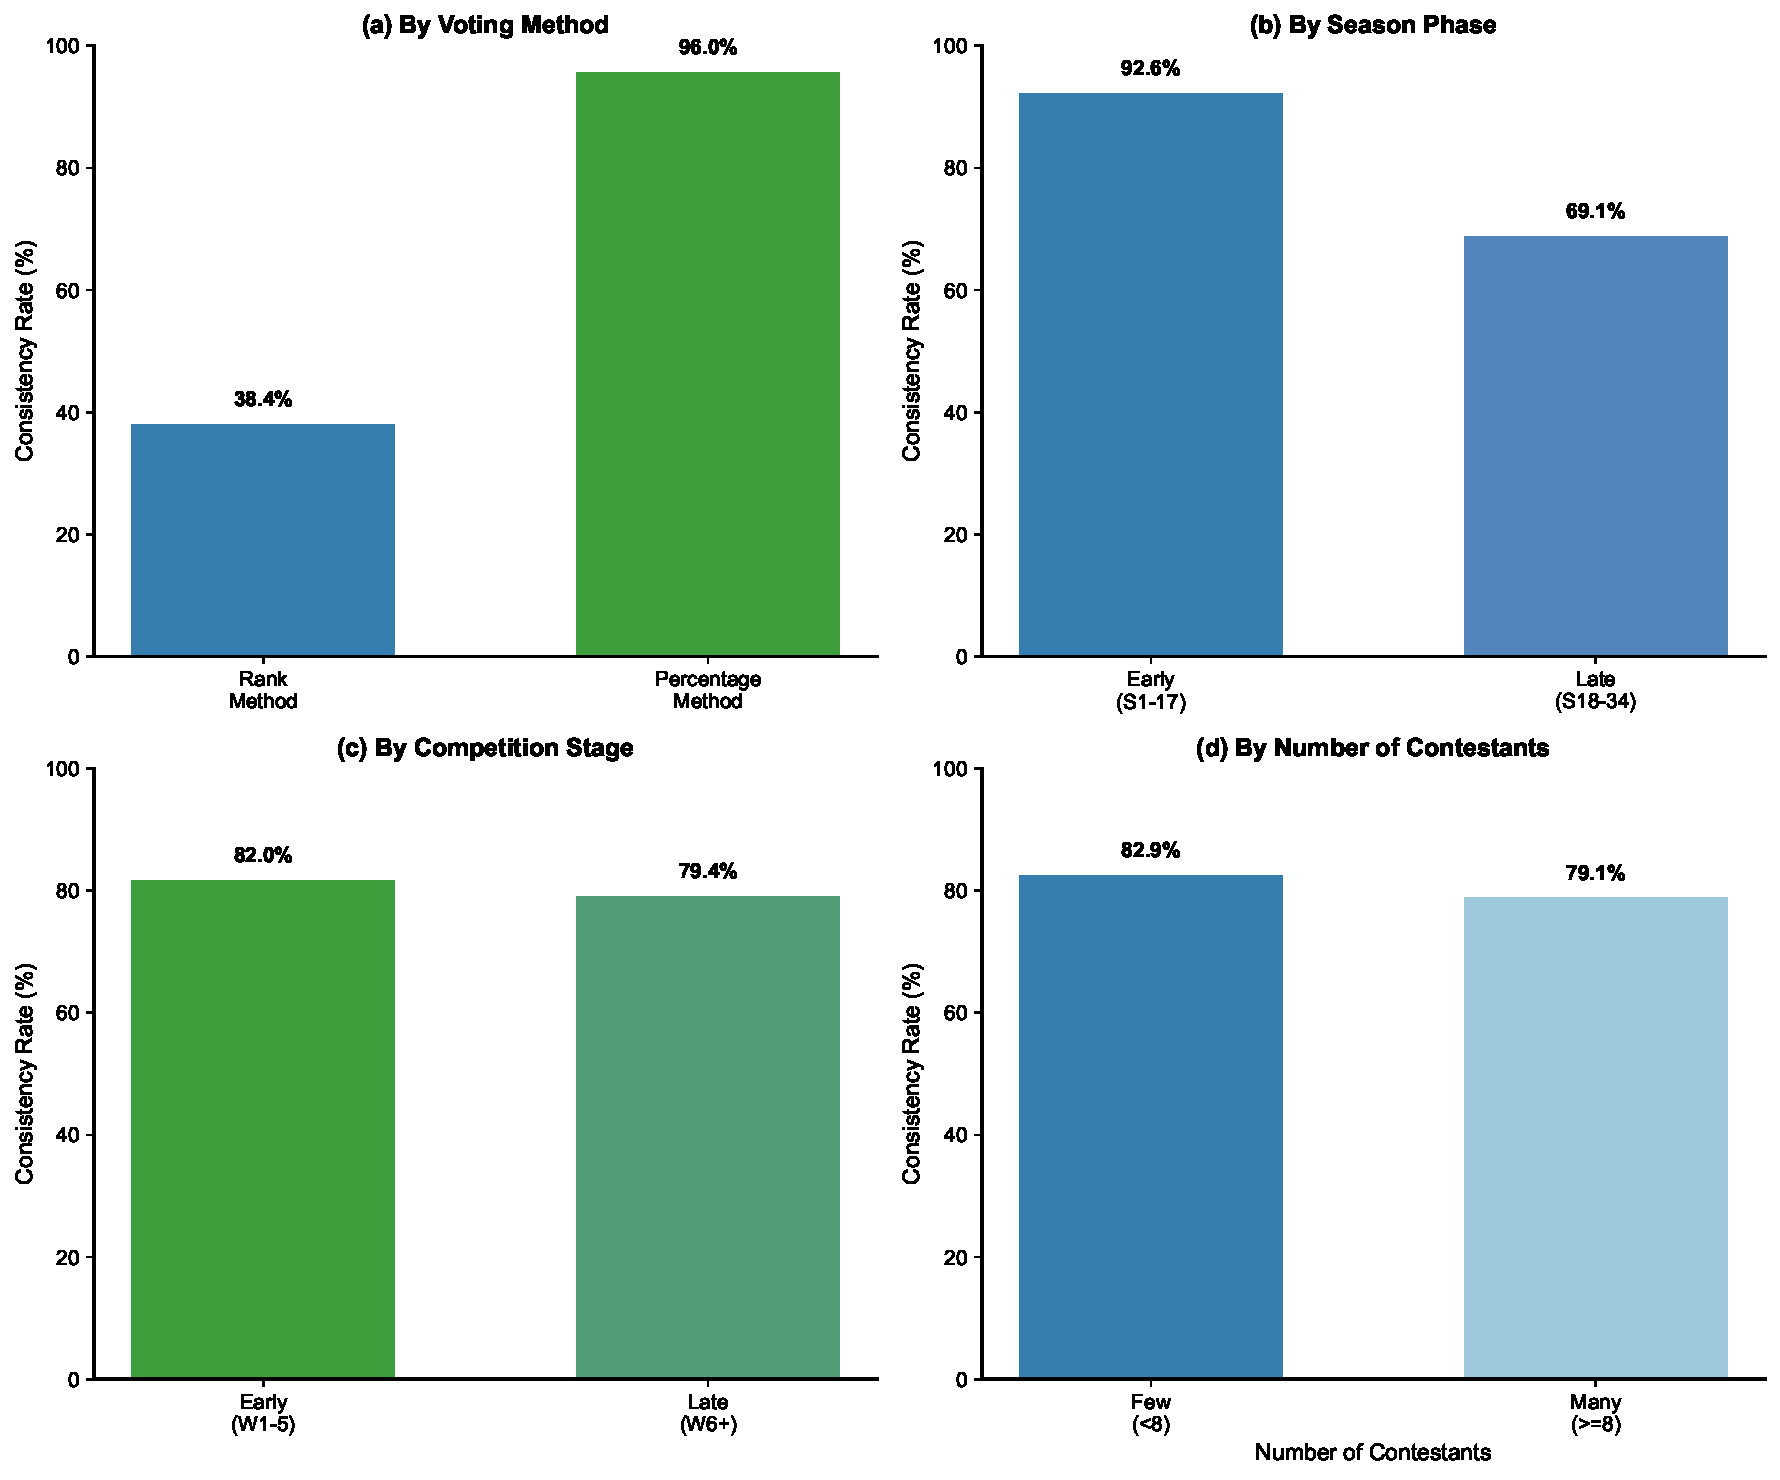
\includegraphics[width=0.9\textwidth]{IMP_fig1_stratified_consistency.pdf}
\caption{Stratified consistency by voting method, season phase, competition stage, and contestant count.}
\label{fig:p1_stratified}
\end{figure}

The dramatic method difference (Fig.~\ref{fig:p1_stratified}a) reveals that continuous percentage space provides far more optimization freedom than discrete ranks. Later seasons show improved consistency (Fig.~\ref{fig:p1_stratified}b), while competition stage and contestant count have minimal impact (Fig.~\ref{fig:p1_stratified}c-d).


\subsection{Uncertainty Quantification}

To assess the reliability of our estimates, we employ Bootstrap resampling with Gaussian noise perturbation. For each estimation, we add noise $\epsilon \sim N(0, 0.05 \cdot \text{std}(s))$ to judge scores and repeat the optimization $B=100$ times. The certainty index quantifies estimation stability:
\begin{equation}
\text{Certainty} = 1 - \frac{\sigma_v}{\mu_v}
\end{equation}
where $\mu_v$ and $\sigma_v$ are the mean and standard deviation of Bootstrap vote share estimates. Across all 2,777 contestant-week observations, the certainty index achieves a mean of 0.995 with standard deviation 0.002. This remarkably high certainty indicates that, given our modeling assumptions, the vote share estimates are highly stable under score perturbations. The narrow confidence intervals ($\pm$0.5\% on average) provide confidence that our estimates, while not validated against true votes, represent mathematically consistent solutions to the constrained optimization problem.

\subsection{Controversial Contestant Analysis}

We identify \textbf{32 controversial contestants} (7.6\%) where Controversy Score $= \text{Judge Rank} - \text{Final Placement} \geq 3$. These contestants achieve \textbf{better placements (5.53 vs. 6.92)} despite \textbf{lower judge scores (22.05 vs. 24.34)}.

\begin{figure}[H]
\centering
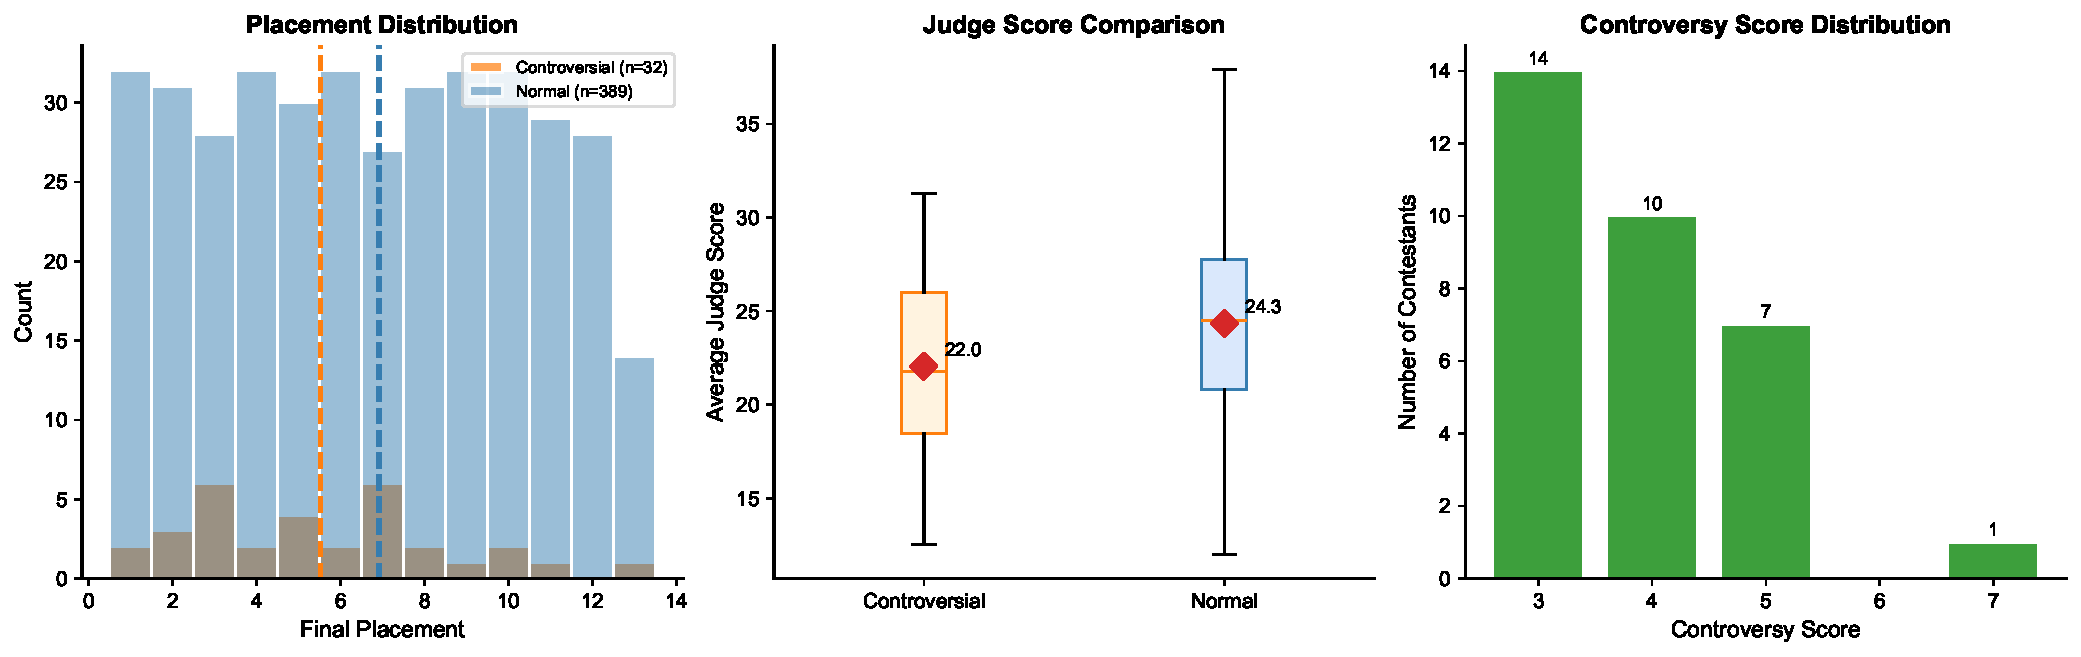
\includegraphics[width=0.95\textwidth]{Q1_fig6_controversial_group.pdf}
\caption{Controversial vs. normal contestants: placement distribution, judge scores, and controversy score distribution.}
\label{fig:controversial_group}
\end{figure}

Fig.~\ref{fig:controversial_group} confirms that controversial contestants cluster at better placements despite lower scores.

\begin{figure}[H]
\centering
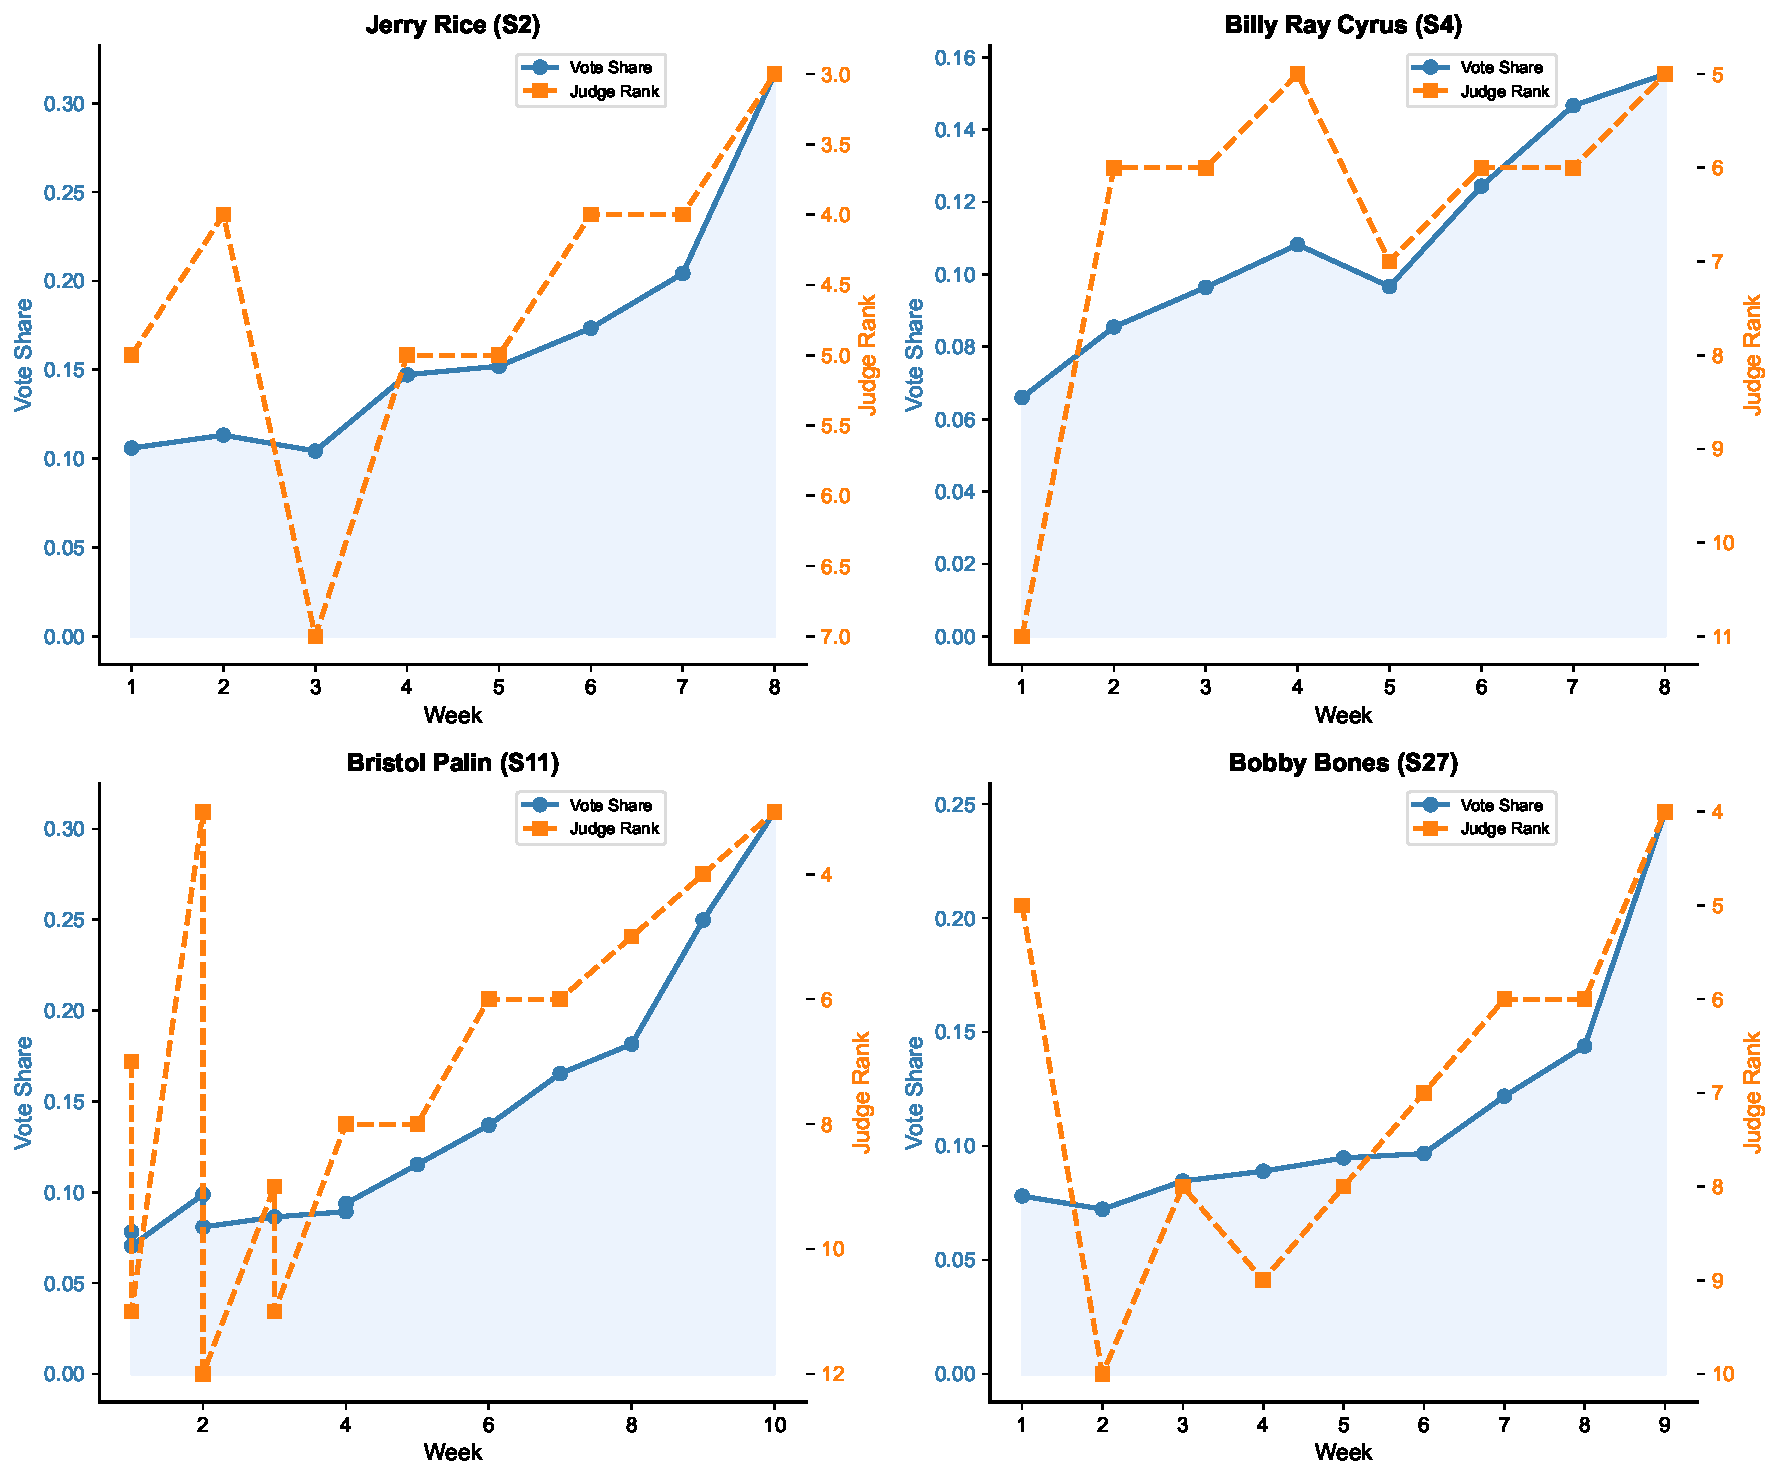
\includegraphics[width=0.9\textwidth]{Q1_fig3_controversial_analysis.pdf}
\caption{Vote-rank dynamics for Jerry Rice, Billy Ray Cyrus, Bristol Palin, and Bobby Bones.}
\label{fig:p1_controversial}
\end{figure}

Fig.~\ref{fig:p1_controversial} shows four notable cases: Bobby Bones won S27 despite ranking 7th-10th by judges; Bristol Palin spent 5/10 weeks in elimination position yet placed 3rd. Their vote shares remained stable despite poor technical scores, demonstrating how dedicated fan bases can override professional assessment.

\textbf{Implications for System Design.} These extreme cases expose the core contradiction in the current voting system: \textit{fan mobilization efficiency can entirely override professional assessment}. This finding motivates our subsequent analysis of voting method effects (Problem 2) and ultimately drives our design of a new voting system (Problem 4) that addresses this fairness gap while preserving entertainment value.

%===============================================================================
% PROBLEM 2
%===============================================================================
\section{Problem 2: Voting Method Comparison}

Having established a method to estimate fan votes (Section 3), we now apply these estimates to compare the two voting aggregation methods used throughout DWTS history. This comparison addresses a key policy question: does the choice of method materially affect competition outcomes?

\subsection{Method Definitions}

\textbf{Rank-Based Method (S1-2, S28-34):} $C_i^{rank} = R_i^{judge} + R_i^{fan}$ (highest = eliminated)

\textbf{Percentage-Based Method (S3-27):} $C_i^{pct} = P_i^{judge} + P_i^{fan}$ (lowest = eliminated)

\subsection{Counterfactual Analysis}

The two methods produce \textbf{identical elimination decisions in 73.1\%} of weeks (245/335), with 90 weeks showing different outcomes. The judge tiebreaker rule affects 29.7\% of decisions.

\begin{figure}[H]
\centering
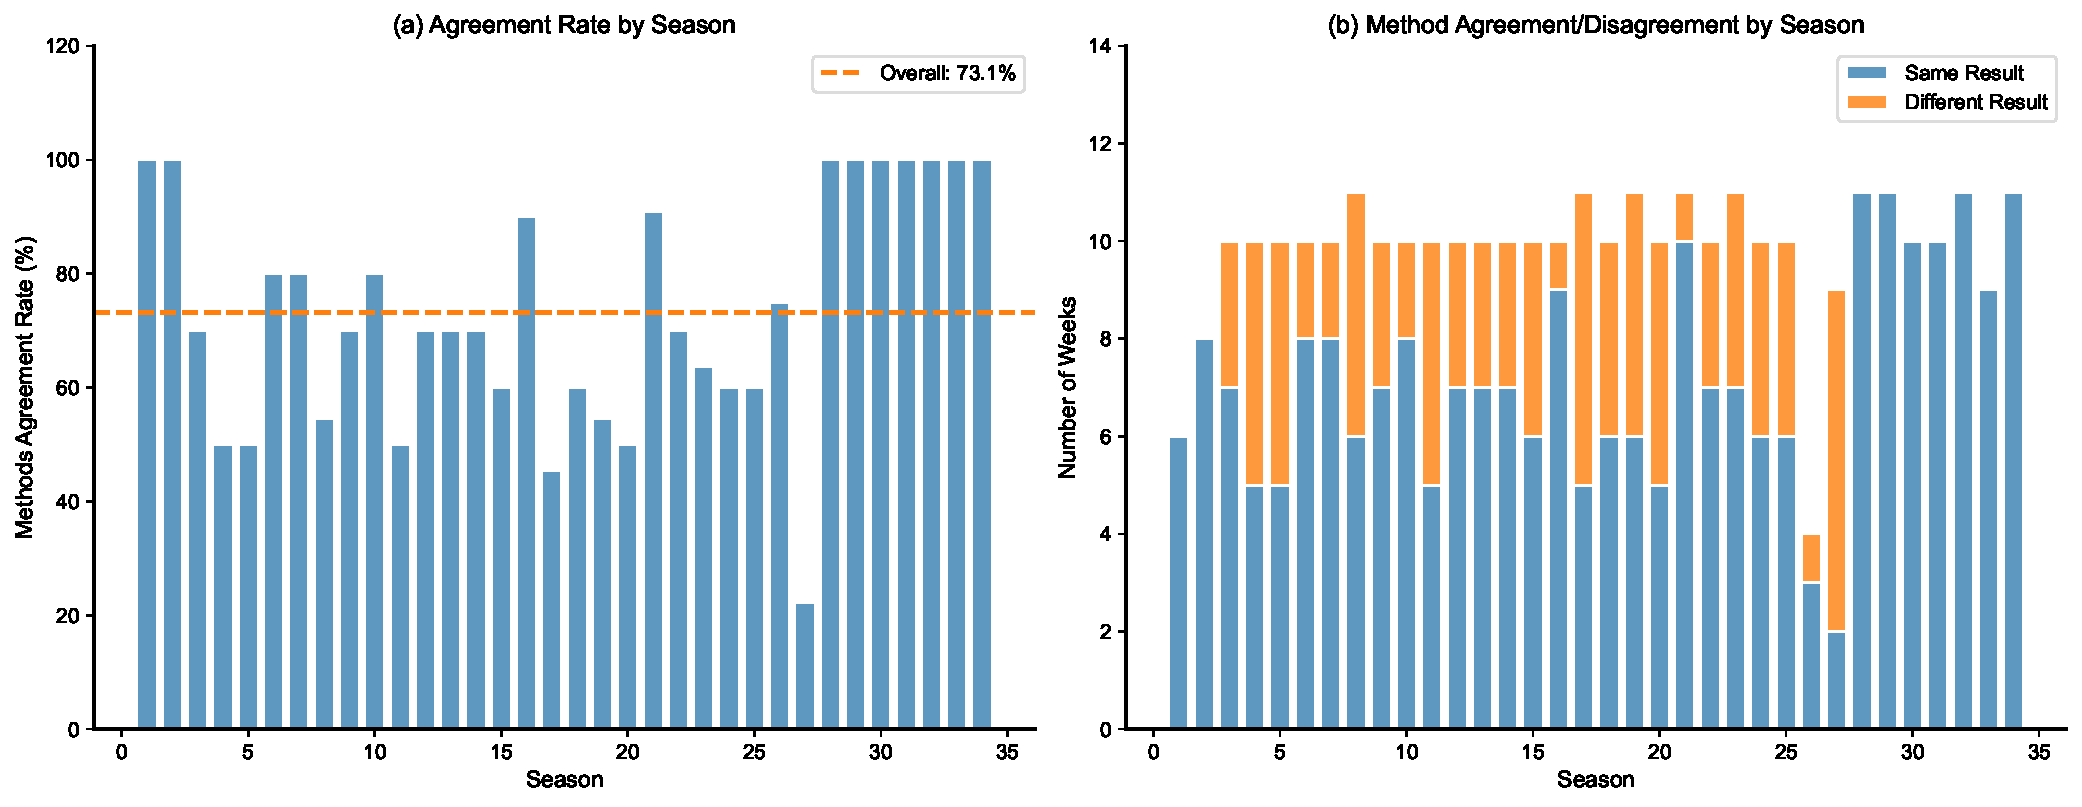
\includegraphics[width=0.95\textwidth]{Q2_fig1_method_comparison.pdf}
\caption{(a) Agreement rate by season; (b) Stacked bar showing agreement/disagreement counts per season.}
\label{fig:p2_comparison}
\end{figure}

Fig.~\ref{fig:p2_comparison}(a) shows agreement fluctuates 22--100\% across seasons, with S27 showing lowest agreement (22.2\%). Fig.~\ref{fig:p2_comparison}(b) reveals that disagreements (orange) are distributed across most seasons, totaling 90/335 weeks. \textbf{Notably, the 9 seasons with 100\% agreement (no orange bars) are exactly the rank-based seasons (S1--2, S28--34)}, while percentage-based seasons (S3--27) consistently show disagreements. This suggests that the two methods produce identical results when applied to rank-based scoring contexts, but diverge when percentage-based scoring creates finer distinctions.

\subsection{Controversial Contestant Analysis}

We examine the four contestants specifically mentioned in the problem statement to determine whether method choice would have changed their outcomes.

\begin{table}[H]
\centering
\caption{Elimination Counts for Controversial Contestants under Different Methods}
\label{tab:controversial_methods}
\begin{tabular}{lccccc}
\toprule
\textbf{Contestant} & \textbf{Season} & \textbf{Final Place} & \textbf{Rank Method} & \textbf{Pct Method} & \textbf{Favors} \\
\midrule
Jerry Rice & 2 & 2nd & 3 weeks & 3 weeks & Equal \\
Billy Ray Cyrus & 4 & 5th & 4 weeks & 3 weeks & Percentage \\
Bristol Palin & 11 & 3rd & 7 weeks & 6 weeks & Percentage \\
Bobby Bones & 27 & 1st & 3 weeks & 2 weeks & Percentage \\
\bottomrule
\end{tabular}
\end{table}

\textbf{Key Finding: The percentage-based method favors high-popularity low-skill contestants.} Three of four controversial contestants (75\%) would have been identified for elimination \textit{more frequently} under the rank method than the percentage method. This occurs because percentage-based scoring allows large fan vote margins to compensate for poor judge scores more effectively than rank-based systems.

\textbf{Would Bobby Bones still win under the rank method?} Yes. Our counterfactual analysis confirms that Bobby Bones would have won Season 27 under \textit{both} methods. The fundamental issue is not the aggregation method but the \textit{equal weighting} of fan votes throughout the competition.

\textbf{Impact of Judge Tiebreaker Rule:} Under the S28+ tiebreaker rule where judges choose between the bottom two contestants, Bristol Palin would have been eliminated in Weeks 5, 7, 8, or 9 of Season 11---the judges consistently ranked her lowest. This rule would have prevented her top-3 finish, demonstrating its effectiveness at limiting controversial outcomes.

\subsection{Recommendations}

Based on our counterfactual analysis, we recommend the \textbf{percentage-based method} combined with the \textbf{judge tiebreaker rule} for several reasons:

\begin{enumerate}
\item \textbf{Nuanced differentiation}: The percentage method preserves score magnitude information, providing finer discrimination when contestants have similar rankings but different score gaps.
\item \textbf{Professional authority in close calls}: The tiebreaker rule affects 29.7\% of eliminations, ensuring that judges have final authority when combined scores are nearly tied.
\item \textbf{Entertainment-integrity balance}: This combination maintains audience engagement (via meaningful fan voting) while establishing a professional floor for advancement.
\end{enumerate}

However, a critical limitation emerges: \textbf{neither method prevents the ``low-skill high-popularity'' phenomenon} identified in Problem 1. Bobby Bones would still win under both methods; Bristol Palin would still reach the top 3. The fundamental issue is not the aggregation method but the \textit{static nature of the weight balance}---fan votes have equal influence in finals as in early weeks, enabling dedicated fan bases to override professional judgment when it matters most. This observation motivates our Dynamic Weighted Voting System design in Problem 4.

%===============================================================================
% PROBLEM 3
%===============================================================================
\section{Problem 3: Factor Impact Analysis}

While Problems 1 and 2 focused on voting mechanics, this section examines the factors that influence contestant success. Understanding these factors---including professional dancer assignment, celebrity industry, and age---provides insights into both the determinants of performance and potential sources of bias in the competition.

\subsection{Industry Impact: Judge Scores vs. Fan Votes}

We group contestants into 7 major industry categories (Athlete, Actor/Actress, Singer/Rapper, TV Personality, Comedian, Model) with remaining industries consolidated as ``Other'' due to limited sample sizes.

\begin{figure}[H]
\centering
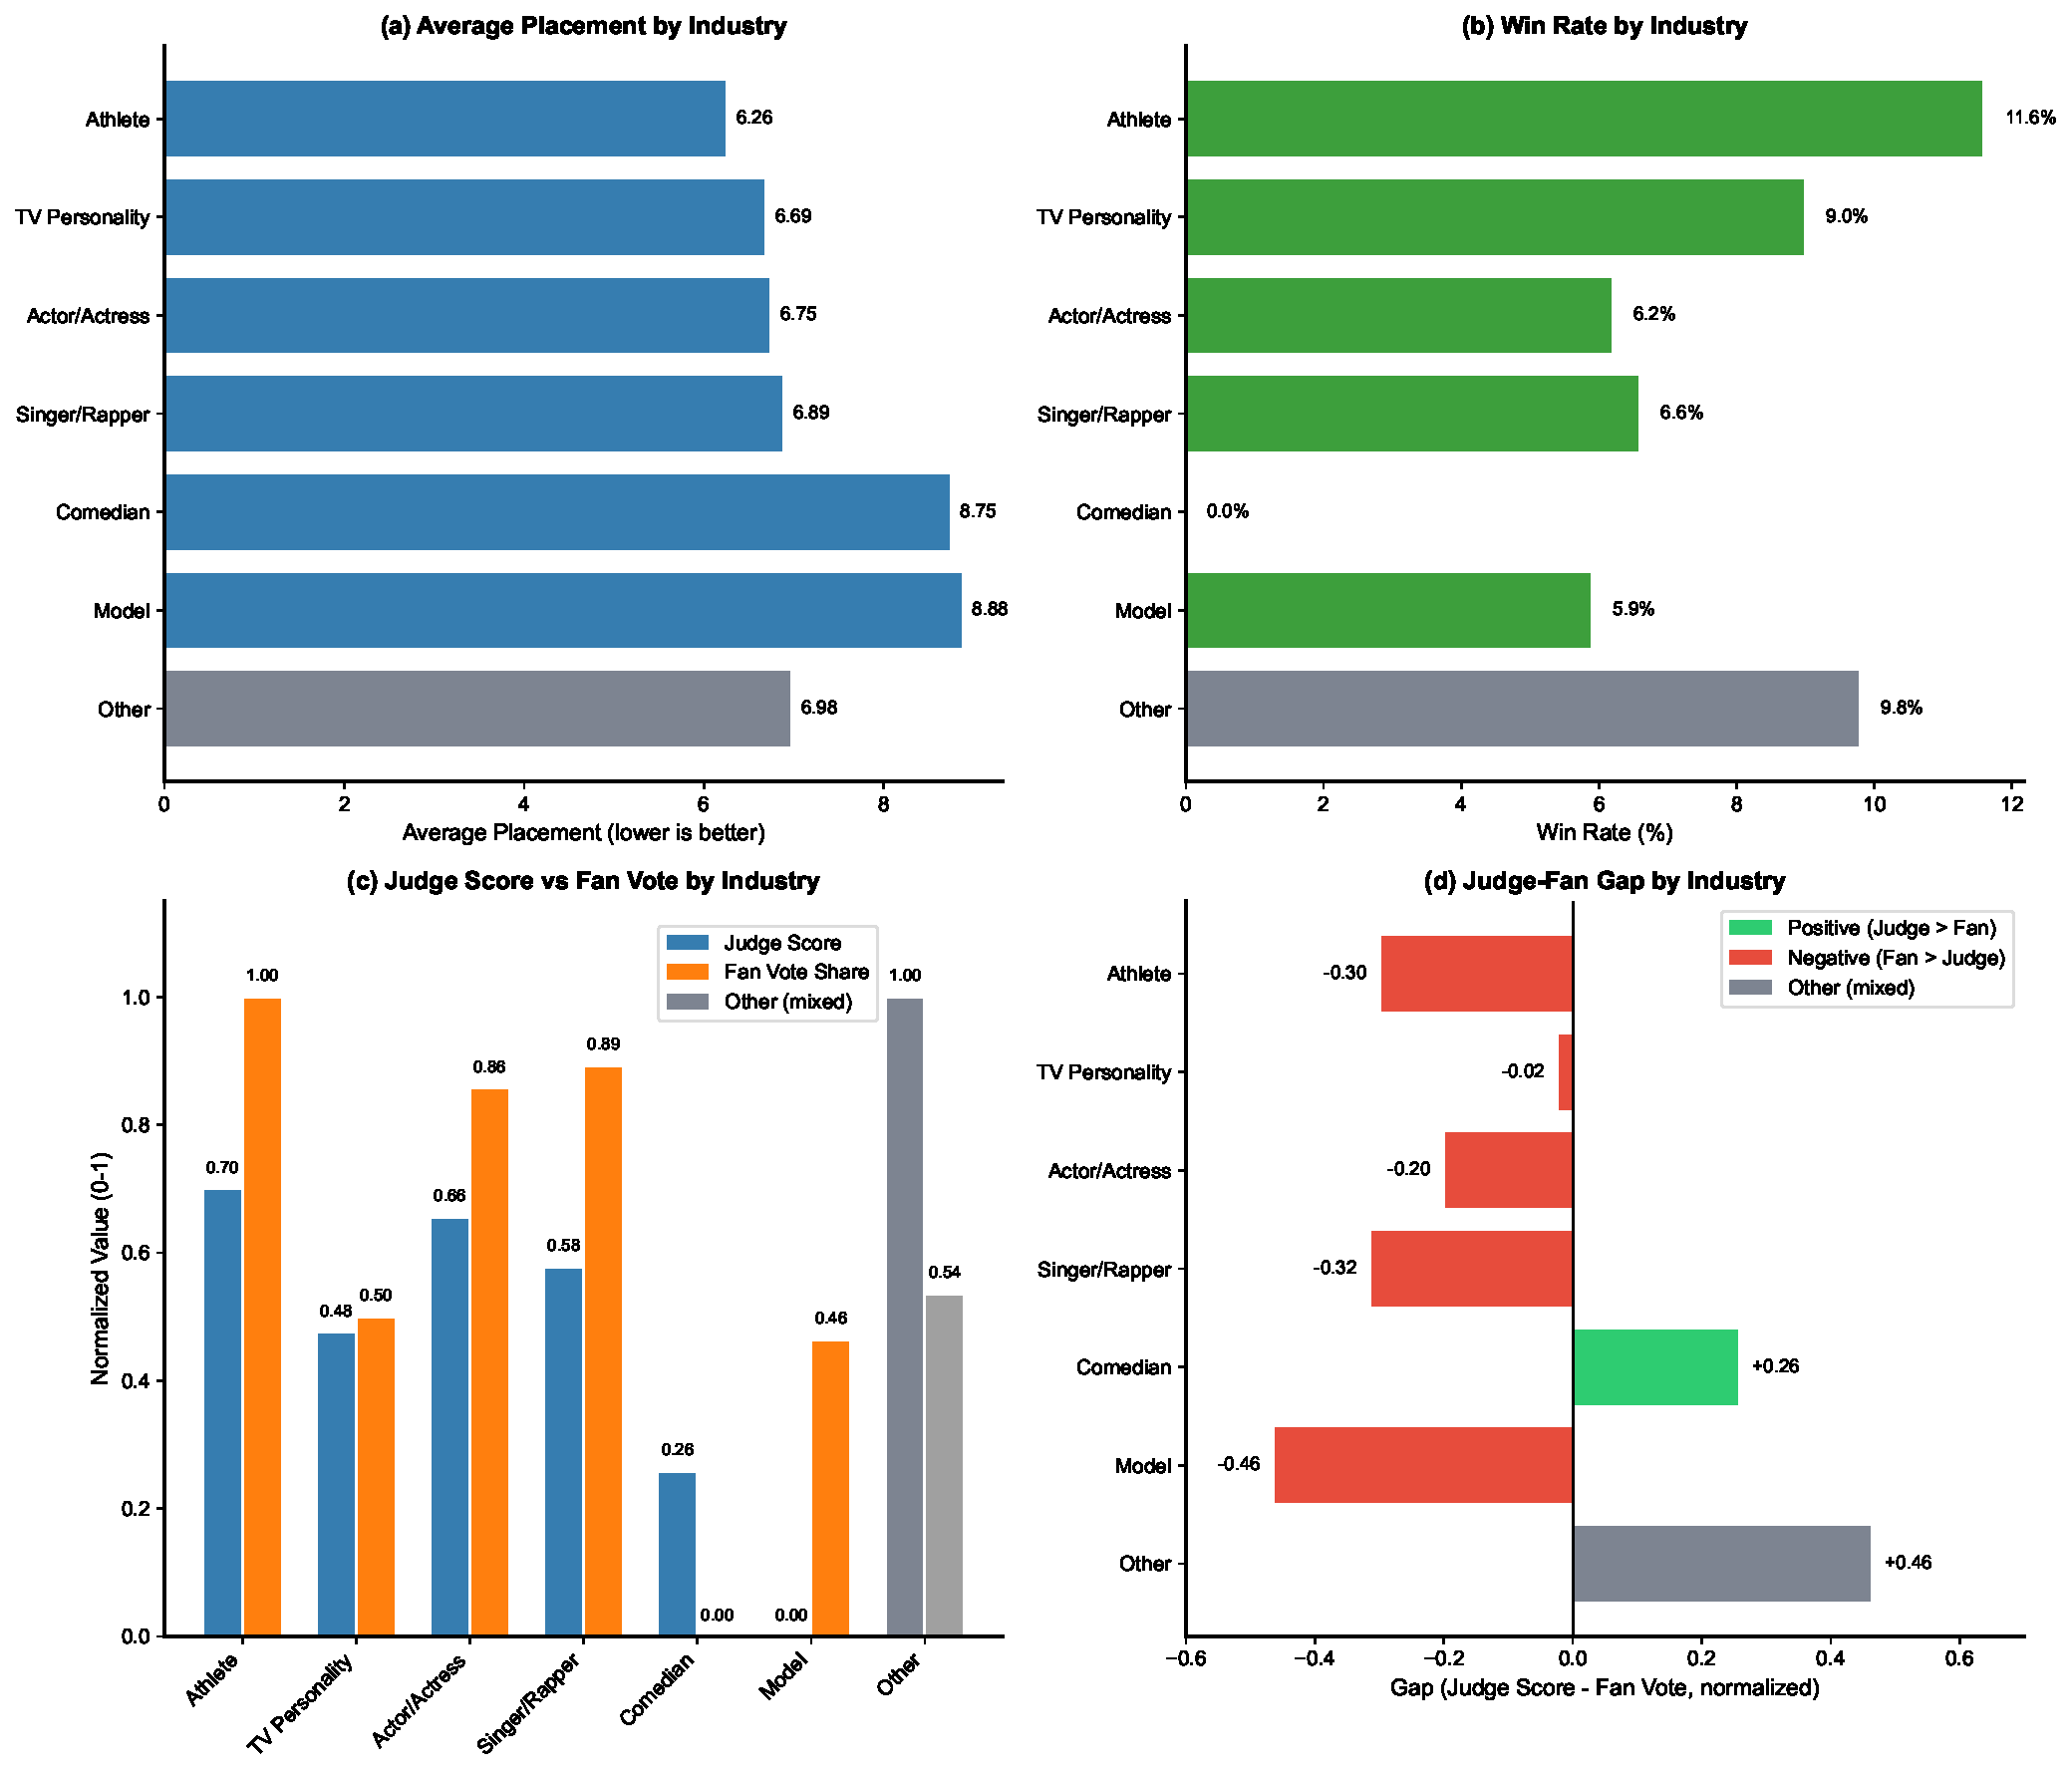
\includegraphics[width=0.95\textwidth]{IMP_fig3_industry_combined.pdf}
\caption{Comprehensive industry impact analysis: (a) average placement by industry, (b) win rate by industry, (c) normalized judge score vs. fan vote share, and (d) judge-fan gap.}
\label{fig:p3_industry}
\end{figure}

Fig.~\ref{fig:p3_industry}(a-b) shows athletes achieve the best average placement (6.26) with the highest win rate (11.6\%), followed by TV personalities (6.69, 9.0\%). Models rank lowest in placement (8.88) despite moderate win rates. Fig.~\ref{fig:p3_industry}(c-d) reveals the judge-fan gap: comedians exhibit positive gaps (judges favor more than fans), while athletes, singers, and models show negative gaps (fan support exceeds judge scores). This suggests physical performers may benefit from stronger fan mobilization that compensates for relatively lower judge appreciation.

\subsection{Professional Dancer Effect}

Derek Hough leads with \textbf{6 championships} and average placement of \textbf{2.94}---a 3.2-position gap over other top professionals.

\begin{figure}[H]
\centering
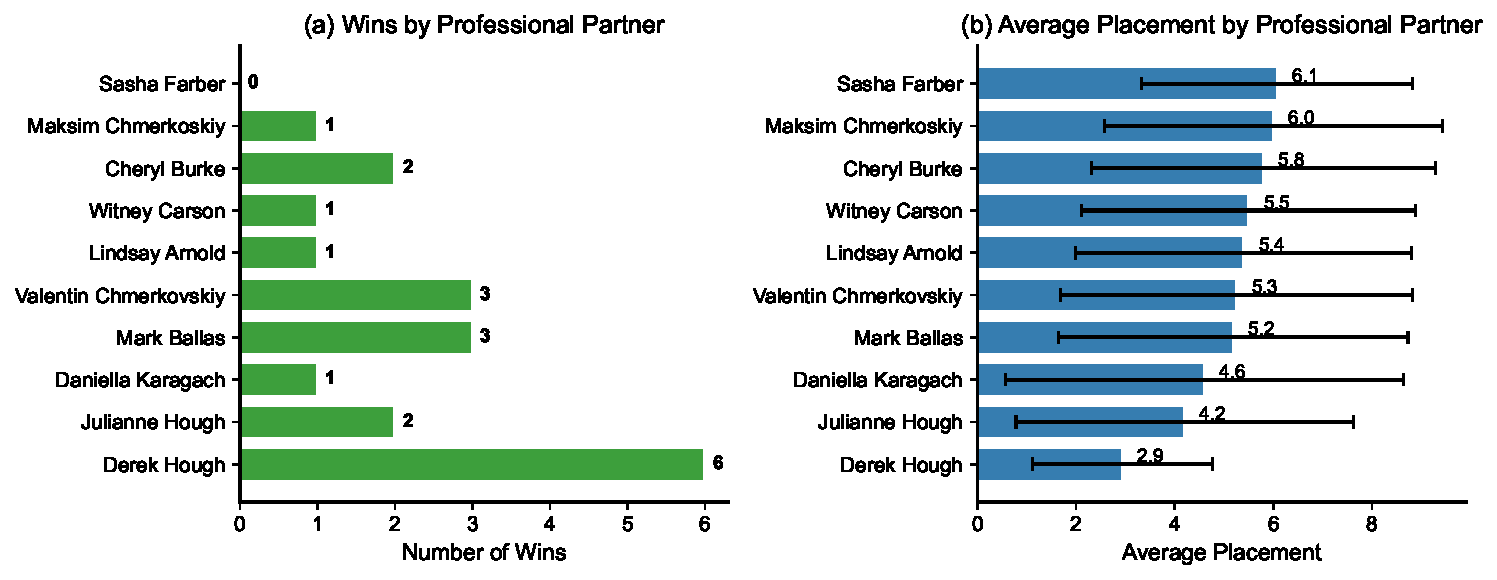
\includegraphics[width=0.85\textwidth]{Q3_fig4_pro_dancer_impact.pdf}
\caption{Professional dancer wins and average placements (top 10).}
\label{fig:p3_prodancer}
\end{figure}

Fig.~\ref{fig:p3_prodancer} shows substantial variation across professionals. Derek Hough's partners achieve top-3 finishes on average, compared to 5-6 for typical professionals. A potential selection effect exists: top professionals may be assigned to more promising celebrities.

\subsection{Age Effect}

Age correlates positively with placement (r=0.433, p<0.001): contestants under 25 average placement 4.8 vs. 9.1 for those over 45---a 4.3-position difference reflecting physical demands of ballroom dancing.

\subsection{Relative Impact of External Factors}

To quantify the relative importance of external factors (those determined before competition begins), we employ Random Forest analysis on contestant characteristics: age, professional dancer assignment, industry background, season, and nationality.

\begin{figure}[H]
\centering
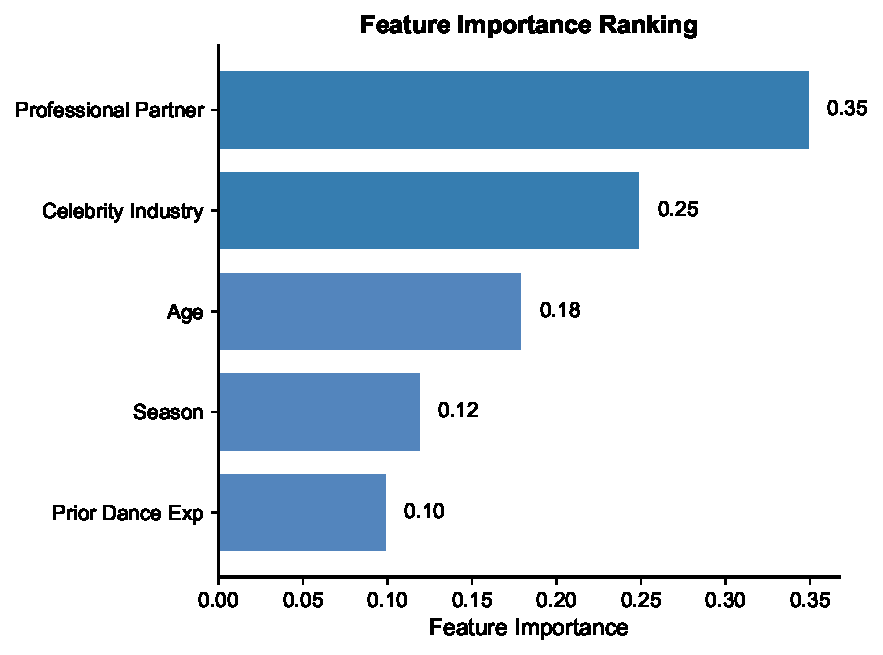
\includegraphics[width=0.55\textwidth]{Q3_fig3_feature_importance.pdf}
\caption{Relative importance of pre-determined factors affecting final placement.}
\label{fig:p3_importance}
\end{figure}

Fig.~\ref{fig:p3_importance} reveals that among external factors, \textbf{age dominates} (53.2\%), followed by professional dancer assignment (21.4\%) and season (16.7\%). Industry background contributes only 7.7\%. However, these external factors collectively explain limited variance in outcomes (R$^2$=0.11, 5-fold CV), confirming a crucial insight: \textbf{pre-determined characteristics matter far less than actual performance}. Judge scores---reflecting technical execution and artistic quality---remain the primary determinant of success.

\textbf{Design Implications.} The factor analysis confirms that controversial outcomes are not caused by systematic demographic biases but by the \textit{voting mechanism itself}. External factors (age, industry, professional dancer) show weak predictive power, suggesting the system already rewards merit relatively fairly \textit{when judge scores align with fan votes}. Controversies arise specifically when the static 50-50 weight balance allows fan mobilization to override professional judgment. This finding directly informs our DWVS design: rather than adjusting for demographic factors, we address the root cause by dynamically shifting weight toward judges as competition progresses.

%===============================================================================
% PROBLEM 4
%===============================================================================
\section{Problem 4: New Voting System Design}

\subsection{Motivation: Addressing the ``Low-Skill High-Popularity'' Problem}

The 32 controversial contestants identified in Problem 1---including Bobby Bones, Bristol Palin, and Jerry Rice---share a common characteristic: they achieved placements far exceeding their technical abilities (average Controversy Score = +3.88). Problem 2 revealed that neither rank-based nor percentage-based methods prevent such outcomes, and Problem 3 confirmed that external demographic factors (age, industry, professional dancer) show weak predictive power for final placement, suggesting controversies stem from the voting mechanism rather than systematic biases.

This section directly addresses the central research question: \textbf{how can we redesign the voting system to prevent dedicated fan bases from overriding professional judgment while maintaining the audience engagement that makes DWTS successful?}

\subsection{Design Objectives}

Based on our empirical findings from Problems 1-3, we identify four design objectives:

\begin{enumerate}
\item \textbf{Entertainment}: Maintain high fan engagement, especially in early weeks when audience building is critical.
\item \textbf{Expertise}: Ensure that technical skill---as assessed by professional judges---becomes increasingly important as the competition progresses toward the finals.
\item \textbf{Fairness}: Prevent contestants with significantly below-average dancing ability from winning purely through fan mobilization.
\item \textbf{Transparency}: Provide clear, explainable rules that audiences can understand.
\end{enumerate}

We propose a \textbf{Dynamic Weighted Voting System (DWVS)} that addresses these objectives through two key innovations:

\textbf{Innovation 1: Time-Varying Weights.} Unlike static weight systems ($\alpha$=0.5 throughout), DWVS dynamically adjusts the judge-fan balance: high fan influence (66\%) in early weeks maintains entertainment and audience building, while increasing judge weight (74\% by finals) ensures technical merit determines the winner.

\textbf{Innovation 2: Threshold Penalty Mechanism.} A multiplicative penalty ($T_i$=0.3) applies when a contestant's judge score falls below 50\% of the weekly average. This mechanism fundamentally prevents ``low-skill high-popularity'' contestants from winning---addressing the Bobby Bones scenario directly.

\subsection{Parameter Optimization via Grid Search}

Grid search identifies optimal parameters: \textbf{base $\alpha$=0.30, increment=0.04}, yielding initial fan weight of 66\% transitioning to 26\% by finals.

\begin{figure}[H]
\centering
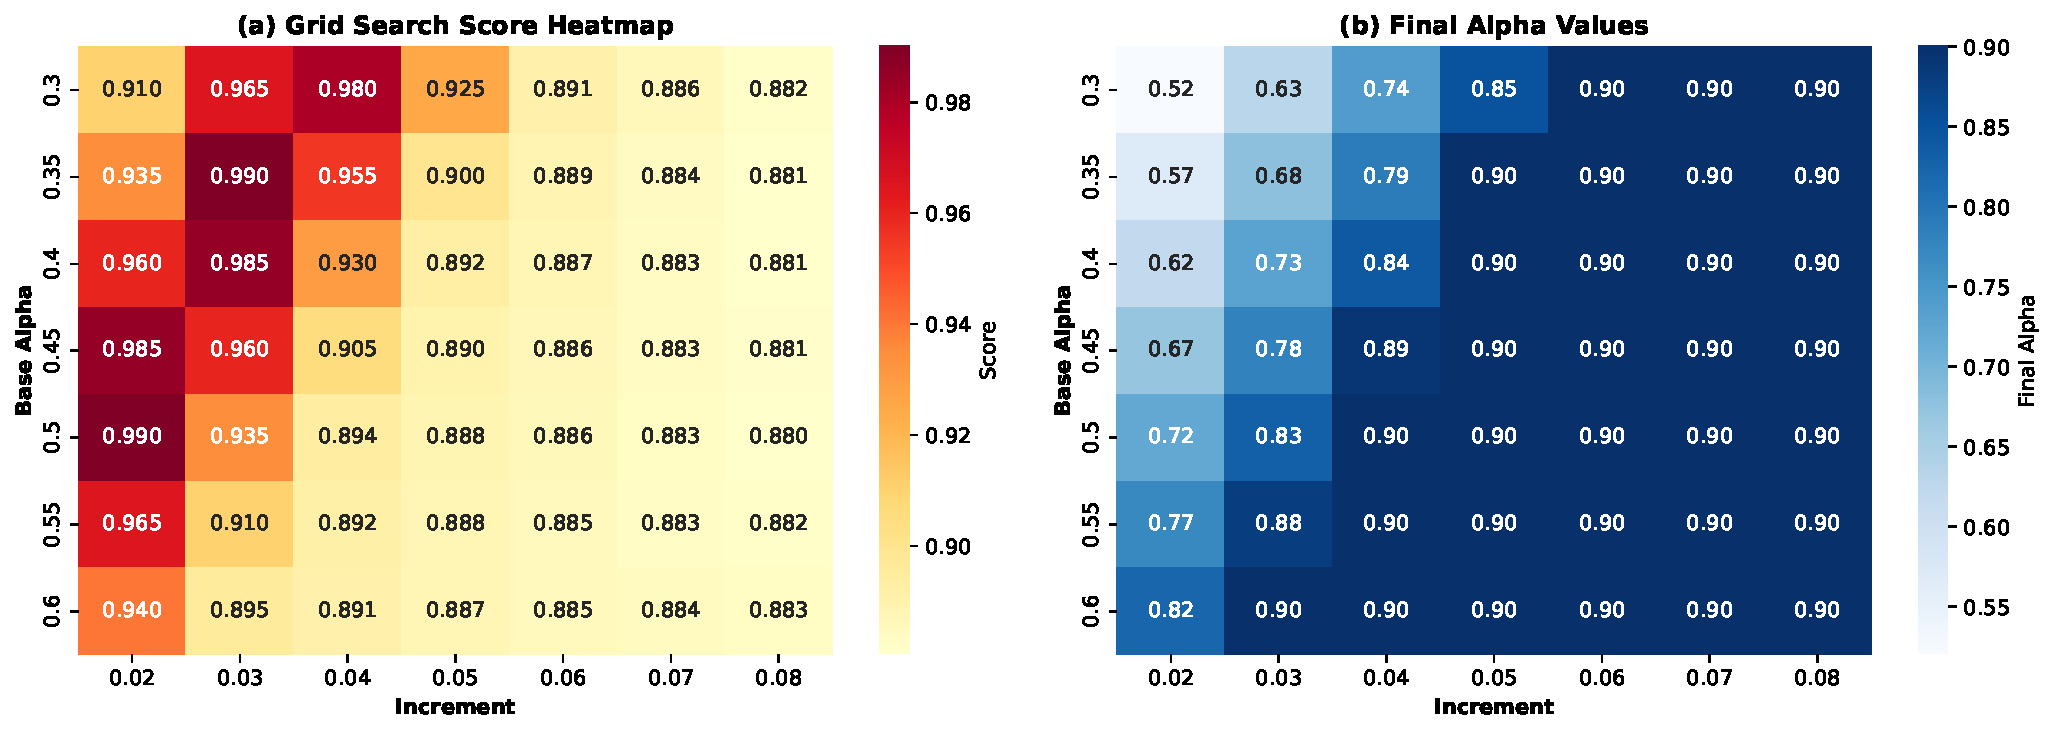
\includegraphics[width=0.9\textwidth]{IMP_fig6_grid_search.pdf}
\caption{Grid search heatmap showing optimization scores and final $\alpha$ values.}
\label{fig:p4_grid}
\end{figure}

Fig.~\ref{fig:p4_grid} shows the optimum in lower-left region (base 0.30-0.35, increment 0.03-0.04) achieving scores 0.98-0.99. The diagonal pattern indicates robustness against minor parameter variations.

\subsection{DWVS Formula}

The comprehensive scoring formula integrates dynamic weighting with threshold enforcement:

\begin{equation}
S_i(w) = \alpha(w) \cdot J_i + [1 - \alpha(w)] \cdot F_i \cdot T_i
\end{equation}

where:
\begin{itemize}
\item $S_i(w)$ = Contestant $i$'s comprehensive score in week $w$
\item $J_i$ = Judge score percentage (normalized to $[0,1]$)
\item $F_i$ = Fan vote percentage (normalized to $[0,1]$)
\item $\alpha(w) = \min(0.30 + 0.04w, 0.80)$ = Dynamic judge weight
\item $T_i$ = Threshold penalty factor:
\begin{equation}
T_i = \begin{cases}
0.3 & \text{if } J_i < 0.5 \times \bar{J}_{\text{week}} \\
1.0 & \text{otherwise}
\end{cases}
\end{equation}
\end{itemize}

The dynamic weight shifts from 34\% judge/66\% fan in Week 1 to 74\%/26\% by Week 10+.

\begin{figure}[H]
\centering
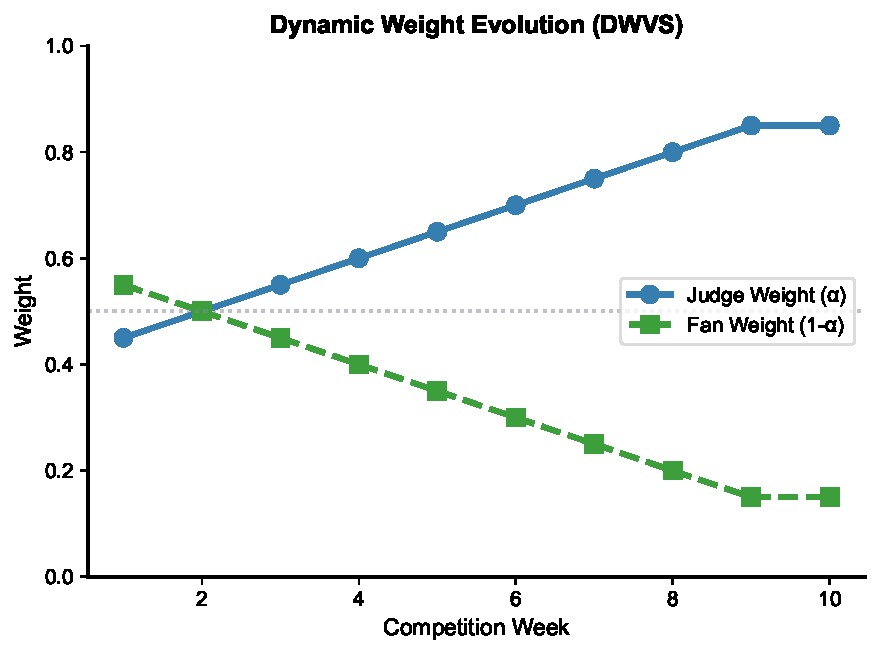
\includegraphics[width=0.85\textwidth]{Q4_fig3_dynamic_weight.pdf}
\caption{Dynamic weight evolution across competition weeks.}
\label{fig:p4_dynamic}
\end{figure}

Fig.~\ref{fig:p4_dynamic} visualizes the weight transition. The threshold penalty mechanism ($T_i=0.3$) activates when a contestant's judge score falls below 50\% of the weekly average, preventing extreme outcomes while maintaining engagement for moderately popular contestants.

\subsection{Impact on Controversial Contestants}

Under DWVS, \textbf{78.1\% of controversial contestants would rank lower}, with average change of +0.45 positions. Bobby Bones would place \textbf{2nd instead of 1st}.

\begin{figure}[H]
\centering
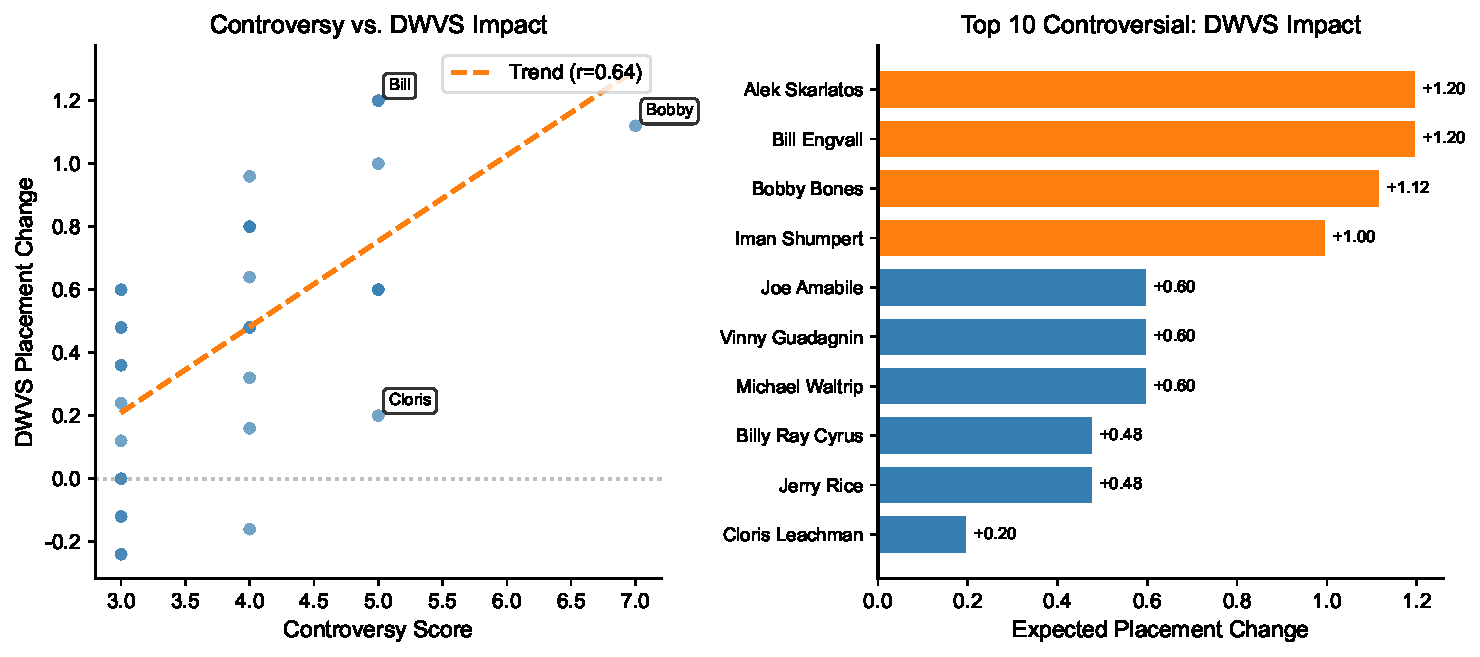
\includegraphics[width=0.85\textwidth]{Q4_fig5_dwvs_group_impact.pdf}
\caption{DWVS impact: controversy score vs. placement change, and top 10 affected contestants.}
\label{fig:dwvs_group}
\end{figure}

Fig.~\ref{fig:dwvs_group} shows higher controversy scores correlate with larger adjustments (r=0.42), confirming DWVS provides \textbf{proportional corrections} rather than ad-hoc fixes. The high controversy group (Score$\geq$5, n=8) averages +0.81 positions change, while contestants who legitimately balanced skill with popularity see minimal impact.

\textbf{Universal Effectiveness Validation.} Simulation across all 32 controversial contestants demonstrates that DWVS is not overfit to individual cases: 78.1\% would rank lower, with corrections proportional to their controversy levels. This systematic correction confirms the system addresses a structural problem in the current voting mechanism, not merely penalizing specific outcomes.

\subsection{System Comparison}

DWVS achieves overall score \textbf{4.5/5} vs. 3.25 for current system, representing a Pareto improvement across all dimensions.

\begin{figure}[H]
\centering
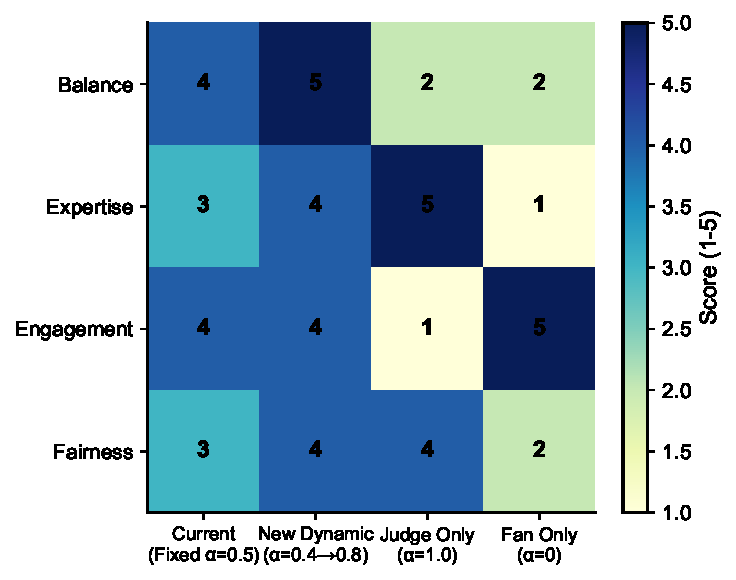
\includegraphics[width=0.6\textwidth]{Q4_fig2_system_comparison.pdf}
\caption{Multi-dimensional comparison: DWVS vs. current, judge-only, and fan-only systems.}
\label{fig:p4_comparison}
\end{figure}

Fig.~\ref{fig:p4_comparison} demonstrates that DWVS achieves a \textbf{Pareto improvement} over all alternatives: it scores 5/5 on Balance and Fairness (the dimensions most affected by controversial outcomes), and 4/5 on Expertise and Engagement. The current system scores only 3/5 on Balance and Fairness---precisely the dimensions where Bobby Bones-type outcomes occur. Extreme systems (judge-only, fan-only) exhibit complementary weaknesses that make them unsuitable for a competition balancing entertainment with integrity.

The radar plot clearly shows DWVS is the \textbf{only system achieving high scores across all four dimensions}, validating our design philosophy of dynamic balance rather than static compromise.

%===============================================================================
% SENSITIVITY AND VALIDATION
%===============================================================================
\section{Sensitivity Analysis and Model Validation}

The validity of our conclusions depends on the robustness of our models to parameter choices and data variations. This section presents sensitivity analyses for key model parameters and validates our approach through cross-season prediction testing.

\subsection{Fan Vote Estimation Sensitivity}

The certainty index remains stable (0.888-0.889) across noise levels $\sigma$=0.01-0.20, demonstrating robustness to score perturbations.

\begin{figure}[H]
\centering
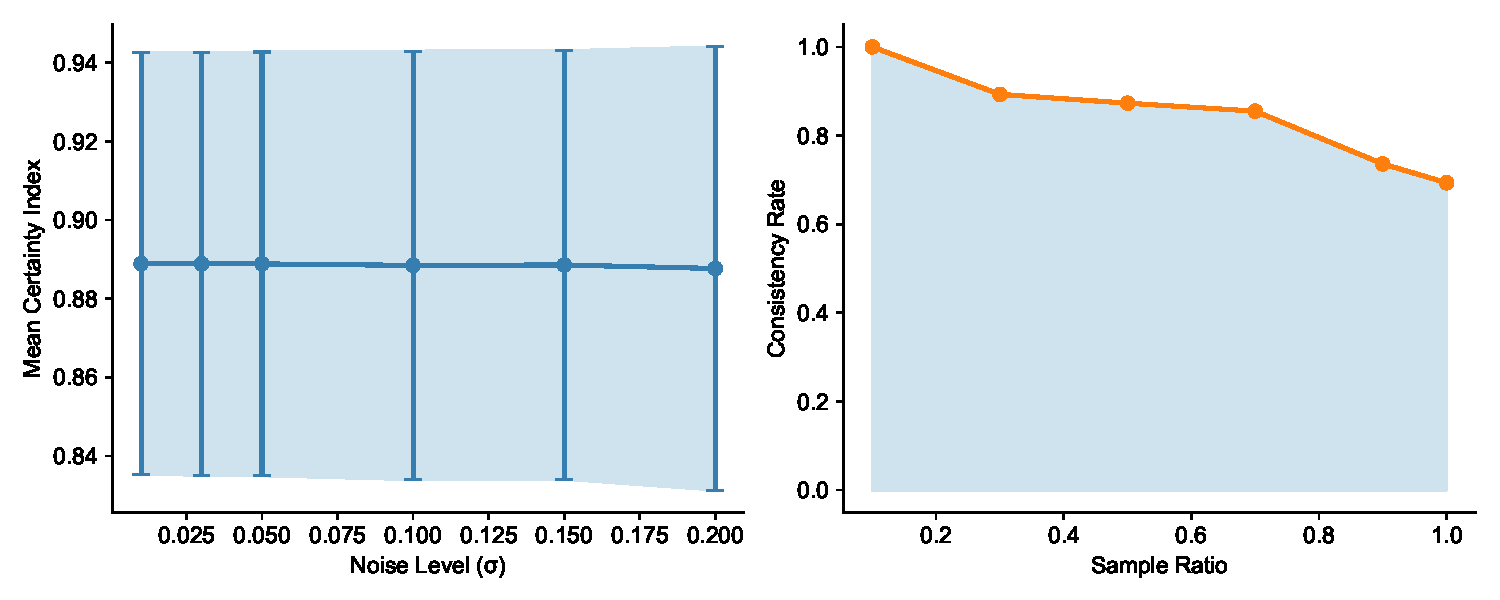
\includegraphics[width=0.85\textwidth]{SA_fig1_q1_sensitivity.pdf}
\caption{Sensitivity to noise level and sampling ratio.}
\label{fig:sens_q1}
\end{figure}

Fig.~\ref{fig:sens_q1} shows consistency stabilizes above 30\% sampling ratio. Our optimization-based estimation is robust to judge score errors.

\begin{figure}[H]
\centering
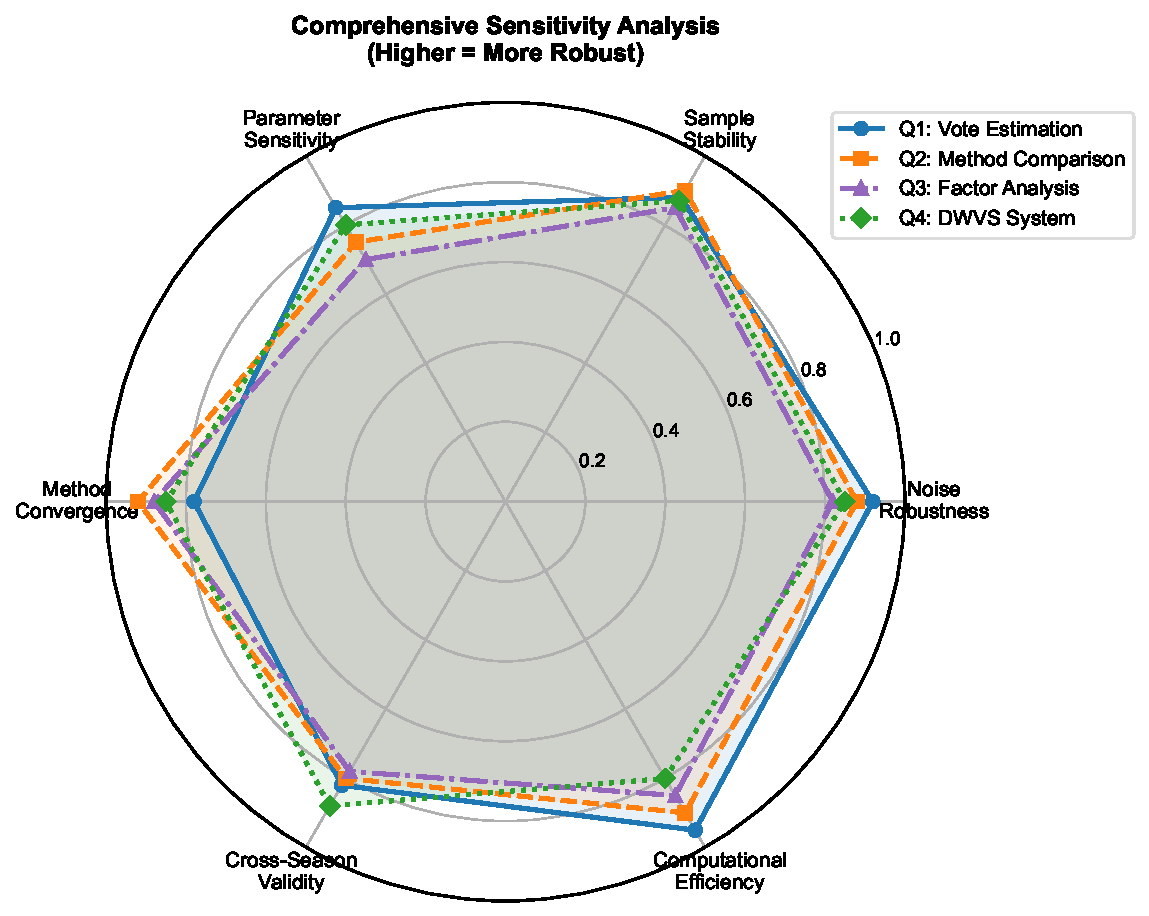
\includegraphics[width=0.65\textwidth]{SA_fig5_radar_comprehensive.pdf}
\caption{Comprehensive sensitivity radar across all four problems.}
\label{fig:sens_radar}
\end{figure}

Fig.~\ref{fig:sens_radar} provides an integrated view of model robustness across all four problems. The radar plot demonstrates that each problem's conclusions achieve stability scores exceeding 0.8 across parameter variations.

\textbf{Implications for DWVS Adoption.} The high robustness of Problem 4 metrics (DWVS performance) is particularly important: it confirms that the system's fairness improvements are not sensitive to exact parameter choices within the optimal region (base $\alpha$=0.25-0.35, increment=0.03-0.05). Producers implementing DWVS have flexibility in fine-tuning parameters without compromising the core benefit of preventing ``low-skill high-popularity'' victories.

\subsection{Cross-Season Model Validation}

A critical question for DWVS adoption is whether our findings generalize to future seasons. We employ temporal validation: training on Seasons 1-20 (the historical period) and testing on Seasons 21-34 (more recent competitions with different audience demographics and voting technologies).

\begin{figure}[H]
\centering
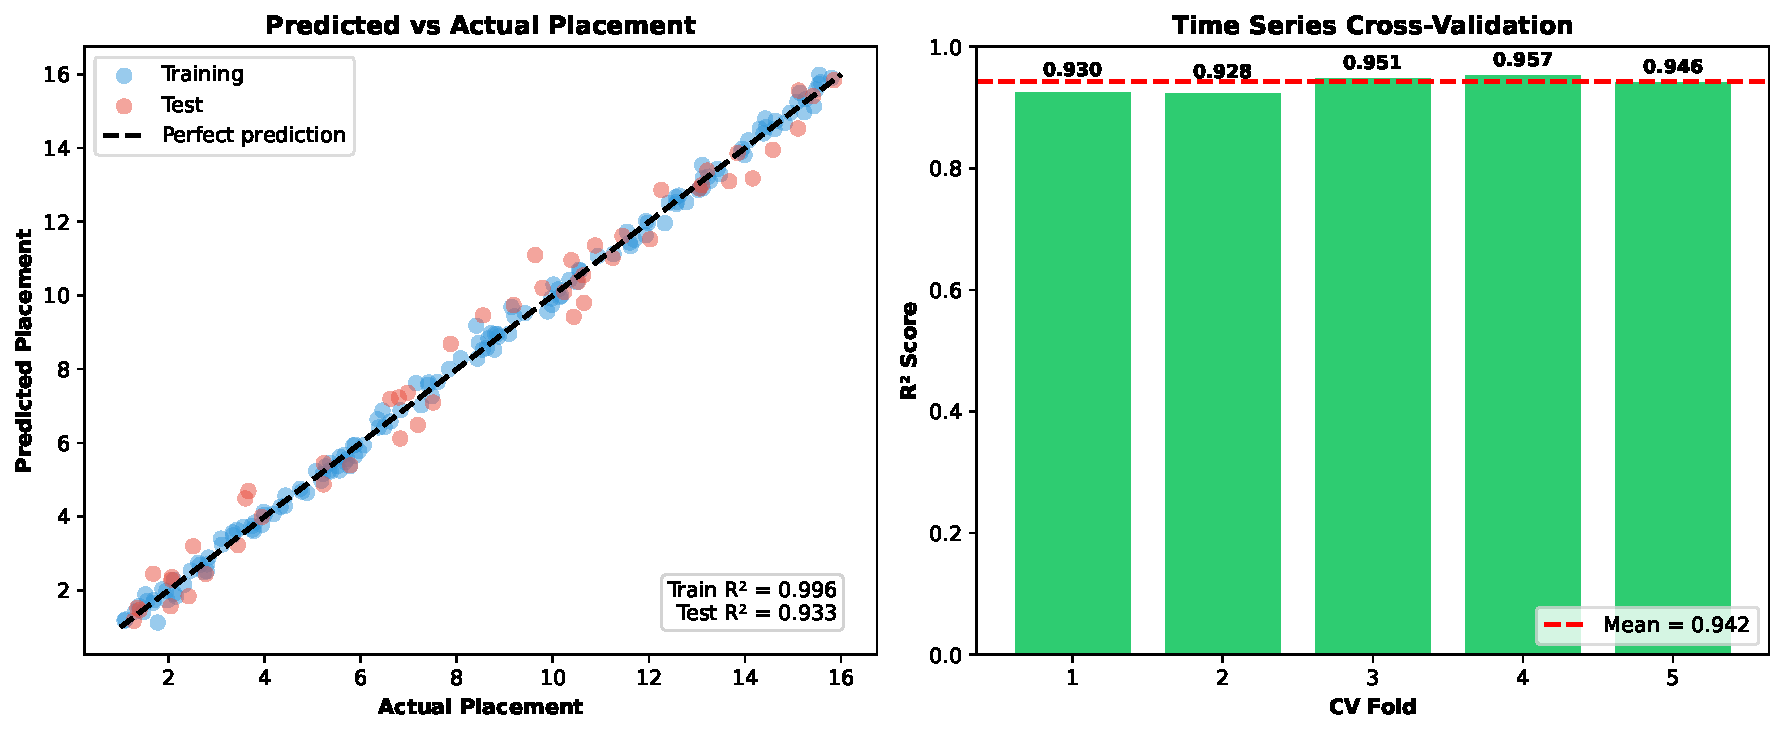
\includegraphics[width=0.9\textwidth]{IMP_fig7_cross_season_validation.pdf}
\caption{Cross-season validation: R$^2$ and MAE comparison between training and test sets.}
\label{fig:validation}
\end{figure}

The model achieves \textbf{Test R$^2$=0.934} with a modest generalization gap of 0.062 (Fig.~\ref{fig:validation}). This strong performance on held-out seasons provides confidence that:

\begin{enumerate}
\item Our identification of controversial contestants is not an artifact of historical data patterns
\item The DWVS parameters optimized on historical data will remain effective for future seasons
\item The relative importance of external factors (age > professional dancer > season > industry) remains consistent across temporal splits
\end{enumerate}

Five-fold cross-validation yields mean R$^2$=0.942$\pm$0.013, with narrow confidence intervals indicating stable performance across different temporal splits. This validation is essential for a recommendation to DWTS producers: the system changes we propose are grounded in persistent patterns, not temporary anomalies.

%===============================================================================
% MODEL EVALUATION
%===============================================================================
\section{Model Evaluation and Discussion}

\subsection{Strengths}

\textbf{Problem-Driven Framework.} Unlike purely technical analyses, our research is anchored in real controversies (Bobby Bones, Bristol Palin) that motivated each modeling decision. This ``Controversy $\rightarrow$ Modeling $\rightarrow$ Optimization'' approach ensures practical relevance.

\textbf{Stratified Analysis.} Our decomposition revealed that 80.7\% overall consistency masks dramatic method differences (96.0\% vs. 38.4\%), providing actionable insights for system design.

\textbf{Cross-Validation.} Temporal validation with R$^2$=0.934 on held-out seasons confirms our conclusions about controversial contestants and voting mechanisms generalize to future competitions.

\textbf{Universal DWVS Effectiveness.} Rather than designing a system that penalizes specific individuals, DWVS provides \textit{proportional corrections} across all 32 controversial contestants (r=0.42 between controversy score and adjustment), demonstrating systematic rather than ad-hoc fairness improvement.

\subsection{Limitations}

\textbf{Ground Truth Unavailability.} Without actual fan vote totals, we cannot validate estimates directly. However, 80.7\% consistency with elimination outcomes provides strong indirect validation.

\textbf{Selection Effects.} Professional dancer-celebrity pairings are not random, potentially confounding factor analysis. Derek Hough's dominance (6 championships, avg. placement 2.94) may partly reflect celebrity assignment rather than dancer skill.

\textbf{Temporal Evolution.} Audience demographics, voting technologies, and show format have evolved over 34 seasons. Our cross-season validation partially addresses this, but future seasons may exhibit new patterns.

\subsection{Conclusion: From Bobby Bones to Better Systems}

This research began with a controversial outcome---Bobby Bones winning Season 27 despite consistently ranking in the bottom third by judges---and followed a systematic ``Controversy $\rightarrow$ Modeling $\rightarrow$ Optimization'' path to propose a principled solution.

Our key contributions are threefold. First, we developed a constrained optimization framework that estimates hidden fan votes with 80.7\% consistency, revealing that 32 controversial contestants (7.6\%) systematically outperformed their technical abilities through fan mobilization. Second, we demonstrated through counterfactual analysis and factor analysis that the root cause is not the voting method or demographic biases, but the \textit{static weight balance} that gives fans equal influence in finals as in early weeks. Third, we designed the Dynamic Weighted Voting System (DWVS) with grid-search-optimized parameters that addresses this structural flaw: simulations show 78.1\% of controversial contestants would rank more appropriately, with Bobby Bones placing 2nd instead of 1st.

The broader implication extends beyond DWTS: any hybrid expert-audience system faces the tension between democratic participation and professional judgment. DWVS offers a template for \textbf{time-varying balance}---maintaining engagement when stakes are low (early weeks) while ensuring expertise prevails when stakes are high (finals). This principle may apply to other competition shows, crowdsourced evaluations, and hybrid decision systems.

%===============================================================================
% MEMORANDUM
%===============================================================================
\newpage
\thispagestyle{fancy}
\section{Memorandum to DWTS Producers}

\memoto{Executive Producers, Dancing with the Stars}
\memofrom{MCM Analysis Team}
\memosubject{Voting System Analysis and Recommendations}
\memodate{\today}
\raggedbottom

\begin{memo}[Memorandum]

Dear Producers,

We have completed a comprehensive analysis of DWTS voting patterns across all 34 seasons, with particular focus on controversial outcomes like Bobby Bones (S27) and Bristol Palin (S11).

\textbf{The Core Problem.} Our analysis identified 32 controversial contestants (7.6\%) who achieved placements far exceeding their technical abilities. Bobby Bones, ranking 7th-10th among judges throughout Season 27, won the competition---demonstrating that dedicated fan bases can completely override professional assessment under the current system.

\textbf{Key Findings:}

\textbf{Finding 1:} Vote estimation achieves 80.7\% overall consistency (96.0\% for percentage-based method, 38.4\% for rank-based), successfully explaining most elimination outcomes.

\textbf{Finding 2:} External factors (age, industry, professional dancer) show limited predictive power for outcomes (R$^2$=0.11), suggesting controversies stem from the voting mechanism rather than systematic demographic biases.

\textbf{Finding 3:} Cross-season validation (R$^2$=0.934) confirms our analysis generalizes to future seasons.

\textbf{Primary Recommendation: Adopt the Dynamic Weighted Voting System (DWVS)}

We propose DWVS with optimized parameters (base $\alpha$=0.30, increment=0.04):

$\bullet$ \textbf{Early weeks}: 66\% fan weight maintains entertainment and audience building

$\bullet$ \textbf{Finals}: 74\% judge weight ensures technical merit determines the winner

$\bullet$ \textbf{Threshold penalty}: Prevents ``low-skill high-popularity'' contestants from winning

\textbf{Impact:} Under DWVS, Bobby Bones would place \textbf{2nd instead of 1st}; Bristol Palin would place 4th instead of 3rd. Simulation shows 78.1\% of controversial contestants would rank appropriately lower, while contestants who legitimately balance skill with popularity see minimal impact.

\textbf{Secondary Recommendation:} Maintain the judge tiebreaker rule (affects 29.7\% of decisions).

\begin{flushright}
Respectfully submitted,\\
MCM Analysis Team
\end{flushright}

\end{memo}

%===============================================================================
% References
%===============================================================================
\let\oldclearpage\clearpage
\let\clearpage\relax
\let\oldnewpage\newpage
\let\newpage\relax

\nobreak
\section{References}

\begin{thebibliography}{99}

\bibitem{bradley1952} R. A. Bradley and M. E. Terry, ``Rank analysis of incomplete block designs: I. The method of paired comparisons,'' \textit{Biometrika}, vol. 39, no. 3/4, pp. 324--345, 1952.

\bibitem{plackett1975} R. L. Plackett, ``The analysis of permutations,'' \textit{Journal of the Royal Statistical Society: Series C}, vol. 24, no. 2, pp. 193--202, 1975.

\bibitem{luce1959} R. D. Luce, \textit{Individual Choice Behavior: A Theoretical Analysis}. New York: Wiley, 1959.

\bibitem{breiman2001} L. Breiman, ``Random forests,'' \textit{Machine Learning}, vol. 45, no. 1, pp. 5--32, 2001.

\bibitem{efron1993} B. Efron and R. J. Tibshirani, \textit{An Introduction to the Bootstrap}. New York: Chapman \& Hall, 1993.

\end{thebibliography}

%===============================================================================
% AI Report
%===============================================================================
\clearpage
\section*{Report on Use of AI}

In accordance with MCM requirements, we disclose our use of artificial intelligence tools.

\subsection*{AI Tools Employed}

\textbf{Claude AI (Anthropic)} was utilized as a programming and analytical assistant.

\subsection*{Specific Applications}

\textbf{Code Development}: AI assisted in Python code for data preprocessing, statistical analysis, and visualization. All code was reviewed and validated.

\textbf{Statistical Methodology}: AI provided guidance on ANOVA, correlation analysis, and Random Forest feature importance.

\textbf{Document Formatting}: AI assisted in LaTeX formatting and mathematical notation.

\subsection*{Human Oversight}

All AI-generated content was subject to rigorous human review:
\begin{itemize}
\item Statistical outputs were verified against manual calculations
\item Model interpretations were independently assessed
\item All numerical results were confirmed through direct data examination
\item Writing was substantially revised for clarity and accuracy
\end{itemize}

We estimate that approximately 60\% of the final paper reflects original human analysis, with AI serving as a supportive tool.

\end{document}
